\documentclass{standalone}
\usepackage{tikz}
\usetikzlibrary{patterns, positioning}
\usepackage[sfdefault]{ClearSans} %% option 'sfdefault' activates Clear Sans as the default text font
\usepackage[T1]{fontenc}

\begin{document}
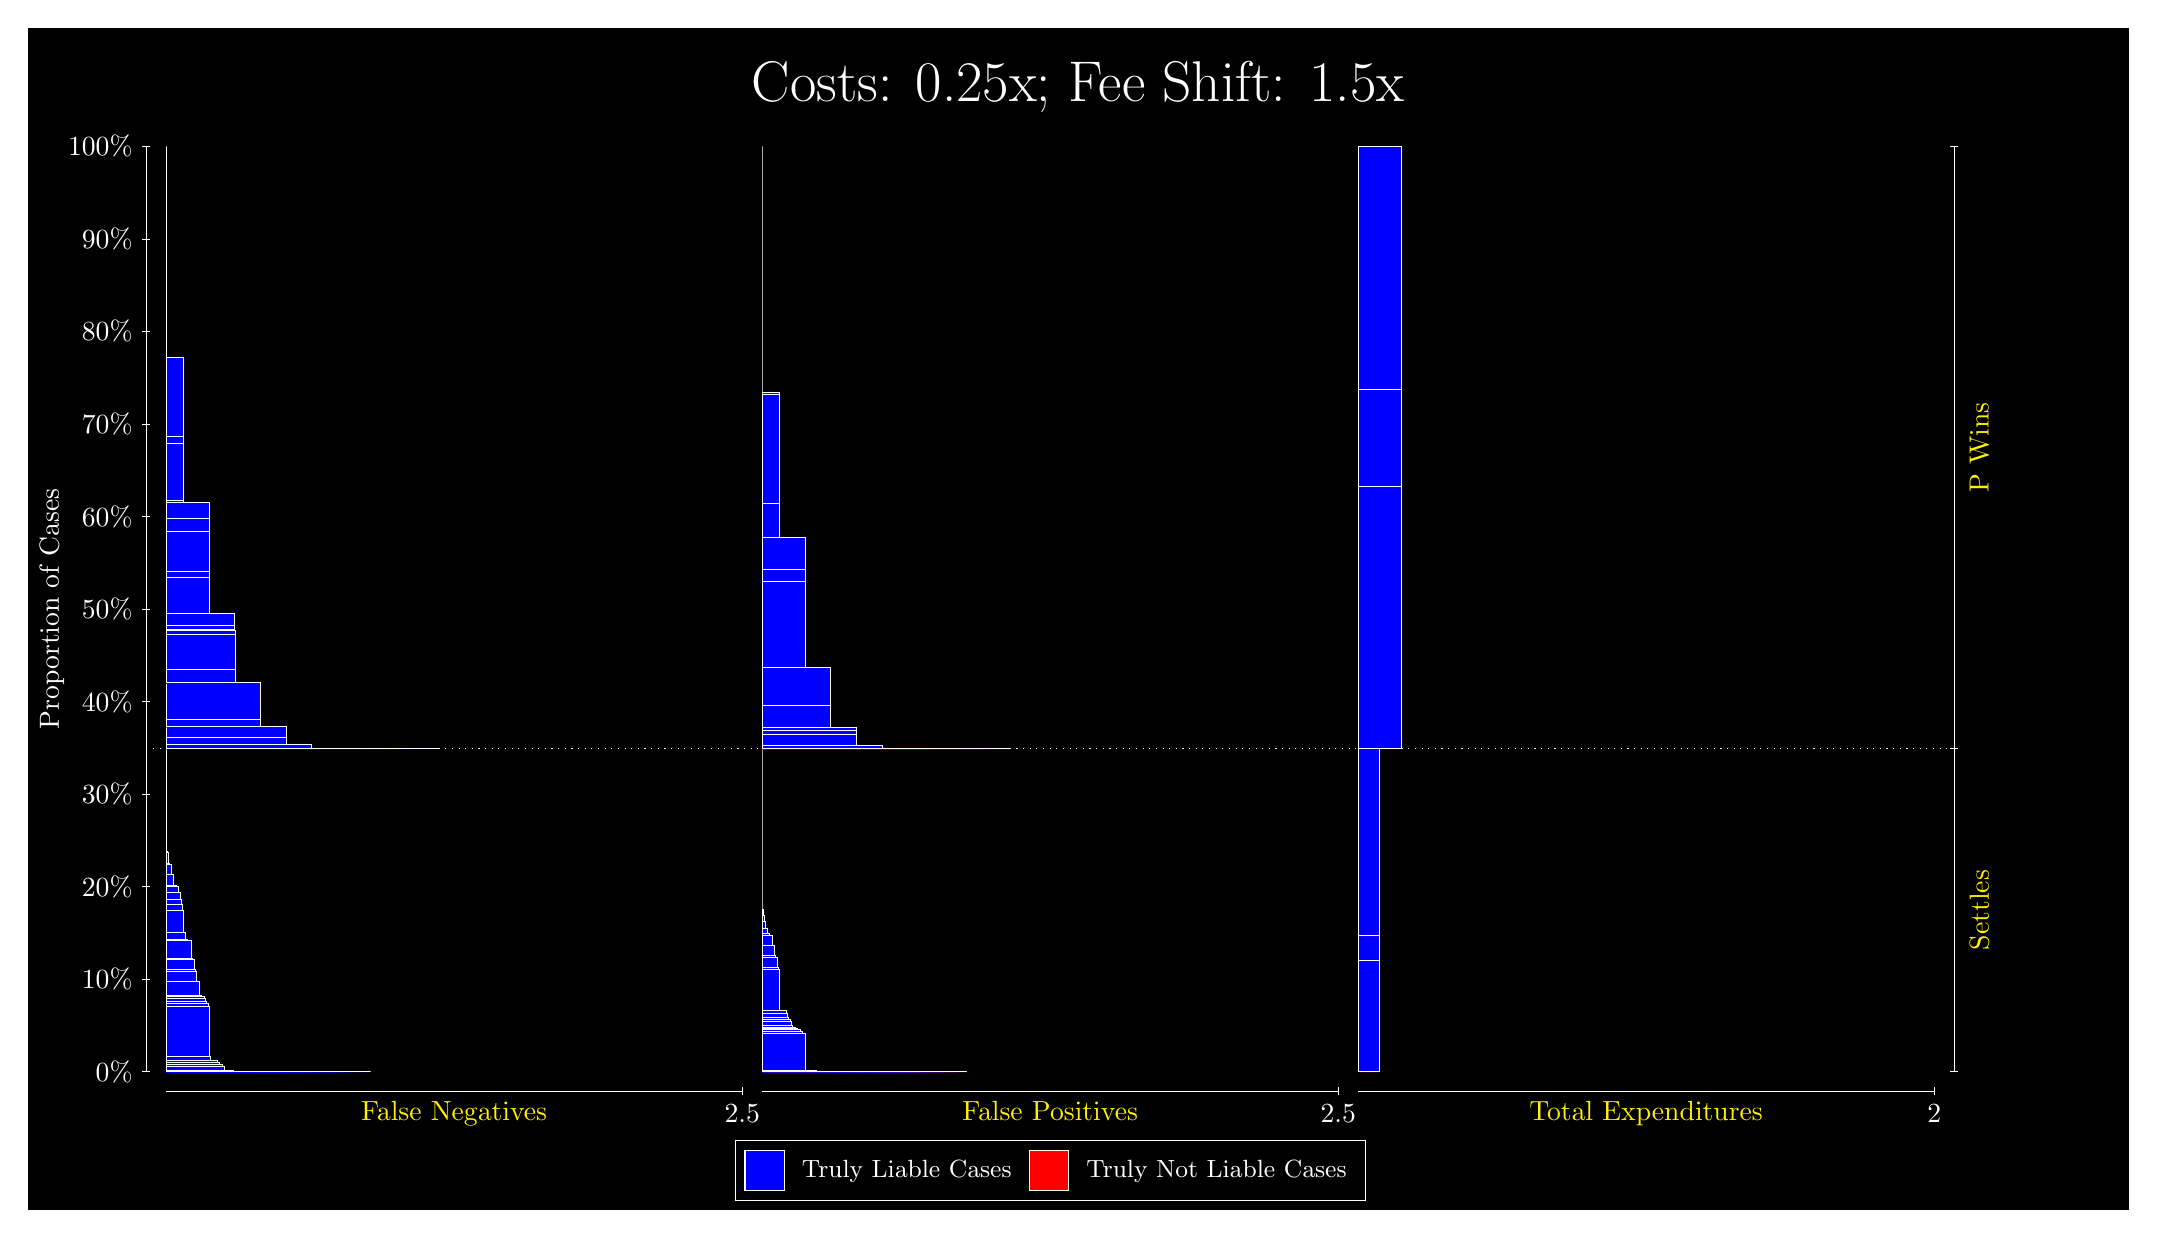
\begin{tikzpicture}
\draw[fill=black] (0,0) rectangle (26.667,15);
\draw[text=white] (0,13.5) rectangle (26.667,15) node[midway] {\huge Costs: 0.25x; Fee Shift: 1.5x};
\draw[white, very thin] (1.5,1.75) -- (1.5,13.5);
\node[rotate=90, text=white, anchor=center] at (0.3, 7.625) {Proportion of Cases};
\draw[white, very thin] (1.45,1.75) -- (1.55,1.75);
\node[text=white, anchor=east] at (1.45, 1.75) {0\%};
\draw[white, very thin] (1.45,2.925) -- (1.55,2.925);
\node[text=white, anchor=east] at (1.45, 2.925) {10\%};
\draw[white, very thin] (1.45,4.1) -- (1.55,4.1);
\node[text=white, anchor=east] at (1.45, 4.1) {20\%};
\draw[white, very thin] (1.45,5.275) -- (1.55,5.275);
\node[text=white, anchor=east] at (1.45, 5.275) {30\%};
\draw[white, very thin] (1.45,6.45) -- (1.55,6.45);
\node[text=white, anchor=east] at (1.45, 6.45) {40\%};
\draw[white, very thin] (1.45,7.625) -- (1.55,7.625);
\node[text=white, anchor=east] at (1.45, 7.625) {50\%};
\draw[white, very thin] (1.45,8.8) -- (1.55,8.8);
\node[text=white, anchor=east] at (1.45, 8.8) {60\%};
\draw[white, very thin] (1.45,9.975) -- (1.55,9.975);
\node[text=white, anchor=east] at (1.45, 9.975) {70\%};
\draw[white, very thin] (1.45,11.15) -- (1.55,11.15);
\node[text=white, anchor=east] at (1.45, 11.15) {80\%};
\draw[white, very thin] (1.45,12.325) -- (1.55,12.325);
\node[text=white, anchor=east] at (1.45, 12.325) {90\%};
\draw[white, very thin] (1.45,13.5) -- (1.55,13.5);
\node[text=white, anchor=east] at (1.45, 13.5) {100\%};

\draw[white, very thin] (24.457,1.75) -- (24.457,13.5);
\draw[white, very thin] (24.407,1.75) -- (24.507,1.75);
\node[anchor=west] at (24.407, 1.75) {};
\draw[white, very thin] (24.407,5.8523) -- (24.507,5.8523);
\node[anchor=west] at (24.407, 5.8523) {};
\draw[white, very thin] (24.407,13.5) -- (24.507,13.5);
\node[anchor=west] at (24.407, 13.5) {};

\draw[white, very thin, fill=blue] (1.75,1.75) rectangle (4.3482,1.75);
\draw[white, very thin, fill=blue] (1.75,1.75) rectangle (4.2018,1.75);
\draw[white, very thin, fill=blue] (1.75,1.75) rectangle (4.0554,1.75);
\draw[white, very thin, fill=blue] (1.75,1.75) rectangle (4.0229,1.75);
\draw[white, very thin, fill=blue] (1.75,1.75) rectangle (3.9091,1.75);
\draw[white, very thin, fill=blue] (1.75,1.75) rectangle (3.8765,1.75);
\draw[white, very thin, fill=blue] (1.75,1.75) rectangle (3.7627,1.75);
\draw[white, very thin, fill=blue] (1.75,1.75) rectangle (3.7302,1.75);
\draw[white, very thin, fill=blue] (1.75,1.75) rectangle (3.6976,1.75);
\draw[white, very thin, fill=blue] (1.75,1.75) rectangle (3.6163,1.75);
\draw[white, very thin, fill=blue] (1.75,1.75) rectangle (3.5838,1.75);
\draw[white, very thin, fill=blue] (1.75,1.75) rectangle (3.5513,1.75);
\draw[white, very thin, fill=blue] (1.75,1.75) rectangle (3.4699,1.75);
\draw[white, very thin, fill=blue] (1.75,1.75) rectangle (3.4374,1.75);
\draw[white, very thin, fill=blue] (1.75,1.75) rectangle (3.4049,1.75);
\draw[white, very thin, fill=blue] (1.75,1.75) rectangle (3.3723,1.75);
\draw[white, very thin, fill=blue] (1.75,1.75) rectangle (3.3236,1.75);
\draw[white, very thin, fill=blue] (1.75,1.75) rectangle (3.291,1.75);
\draw[white, very thin, fill=blue] (1.75,1.75) rectangle (3.2585,1.75);
\draw[white, very thin, fill=blue] (1.75,1.75) rectangle (3.226,1.75);
\draw[white, very thin, fill=blue] (1.75,1.75) rectangle (3.1772,1.75);
\draw[white, very thin, fill=blue] (1.75,1.75) rectangle (3.1447,1.75);
\draw[white, very thin, fill=blue] (1.75,1.75) rectangle (3.1121,1.75);
\draw[white, very thin, fill=blue] (1.75,1.75) rectangle (3.0796,1.75);
\draw[white, very thin, fill=blue] (1.75,1.75) rectangle (3.0471,1.75);
\draw[white, very thin, fill=blue] (1.75,1.75) rectangle (3.0308,1.75);
\draw[white, very thin, fill=blue] (1.75,1.75) rectangle (2.9983,1.75);
\draw[white, very thin, fill=blue] (1.75,1.75) rectangle (2.9657,1.7501);
\draw[white, very thin, fill=blue] (1.75,1.7501) rectangle (2.9332,1.7501);
\draw[white, very thin, fill=blue] (1.75,1.7501) rectangle (2.9007,1.7501);
\draw[white, very thin, fill=blue] (1.75,1.7501) rectangle (2.8844,1.7502);
\draw[white, very thin, fill=blue] (1.75,1.7502) rectangle (2.8519,1.7503);
\draw[white, very thin, fill=blue] (1.75,1.7503) rectangle (2.8194,1.7524);
\draw[white, very thin, fill=blue] (1.75,1.7524) rectangle (2.7868,1.753);
\draw[white, very thin, fill=blue] (1.75,1.753) rectangle (2.7543,1.7535);
\draw[white, very thin, fill=blue] (1.75,1.7535) rectangle (2.738,1.7536);
\draw[white, very thin, fill=blue] (1.75,1.7536) rectangle (2.7218,1.7541);
\draw[white, very thin, fill=blue] (1.75,1.7541) rectangle (2.7055,1.7542);
\draw[white, very thin, fill=blue] (1.75,1.7542) rectangle (2.673,1.7543);
\draw[white, very thin, fill=blue] (1.75,1.7543) rectangle (2.6405,1.7587);
\draw[white, very thin, fill=blue] (1.75,1.7587) rectangle (2.6079,1.7606);
\draw[white, very thin, fill=blue] (1.75,1.7606) rectangle (2.5917,1.7644);
\draw[white, very thin, fill=blue] (1.75,1.7644) rectangle (2.5754,1.7661);
\draw[white, very thin, fill=blue] (1.75,1.7661) rectangle (2.5591,1.7682);
\draw[white, very thin, fill=blue] (1.75,1.7682) rectangle (2.5266,1.7709);
\draw[white, very thin, fill=blue] (1.75,1.7709) rectangle (2.4941,1.8155);
\draw[white, very thin, fill=blue] (1.75,1.8155) rectangle (2.4616,1.8371);
\draw[white, very thin, fill=blue] (1.75,1.8371) rectangle (2.4453,1.8427);
\draw[white, very thin, fill=blue] (1.75,1.8427) rectangle (2.429,1.8627);
\draw[white, very thin, fill=blue] (1.75,1.8627) rectangle (2.4128,1.8658);
\draw[white, very thin, fill=blue] (1.75,1.8658) rectangle (2.3965,1.8895);
\draw[white, very thin, fill=blue] (1.75,1.8895) rectangle (2.3802,1.8912);
\draw[white, very thin, fill=blue] (1.75,1.8912) rectangle (2.3477,1.8929);
\draw[white, very thin, fill=blue] (1.75,1.8929) rectangle (2.3152,1.9374);
\draw[white, very thin, fill=blue] (1.75,1.9374) rectangle (2.2989,2.5823);
\draw[white, very thin, fill=blue] (1.75,2.5823) rectangle (2.2827,2.6118);
\draw[white, very thin, fill=blue] (1.75,2.6118) rectangle (2.2664,2.645);
\draw[white, very thin, fill=blue] (1.75,2.645) rectangle (2.2501,2.675);
\draw[white, very thin, fill=blue] (1.75,2.675) rectangle (2.2339,2.703);
\draw[white, very thin, fill=blue] (1.75,2.703) rectangle (2.2013,2.7207);
\draw[white, very thin, fill=blue] (1.75,2.7207) rectangle (2.1688,2.8985);
\draw[white, very thin, fill=blue] (1.75,2.8985) rectangle (2.1363,3.0288);
\draw[white, very thin, fill=blue] (1.75,3.0288) rectangle (2.12,3.0486);
\draw[white, very thin, fill=blue] (1.75,3.0486) rectangle (2.1037,3.1763);
\draw[white, very thin, fill=blue] (1.75,3.1763) rectangle (2.0875,3.1937);
\draw[white, very thin, fill=blue] (1.75,3.1937) rectangle (2.0712,3.4184);
\draw[white, very thin, fill=blue] (1.75,3.4184) rectangle (2.055,3.4228);
\draw[white, very thin, fill=blue] (1.75,3.4228) rectangle (2.0224,3.4272);
\draw[white, very thin, fill=blue] (1.75,3.4272) rectangle (1.9899,3.5131);
\draw[white, very thin, fill=blue] (1.75,3.5131) rectangle (1.9736,3.7957);
\draw[white, very thin, fill=blue] (1.75,3.7957) rectangle (1.9574,3.8696);
\draw[white, very thin, fill=blue] (1.75,3.8696) rectangle (1.9411,3.9434);
\draw[white, very thin, fill=blue] (1.75,3.9434) rectangle (1.9248,4.0304);
\draw[white, very thin, fill=blue] (1.75,4.0304) rectangle (1.9086,4.0995);
\draw[white, very thin, fill=blue] (1.75,4.0995) rectangle (1.876,4.1171);
\draw[white, very thin, fill=blue] (1.75,4.1171) rectangle (1.8435,4.2536);
\draw[white, very thin, fill=blue] (1.75,4.2536) rectangle (1.811,4.3813);
\draw[white, very thin, fill=blue] (1.75,4.3813) rectangle (1.7947,4.3988);
\draw[white, very thin, fill=blue] (1.75,4.3988) rectangle (1.7785,4.5307);
\draw[white, very thin, fill=blue] (1.75,4.5307) rectangle (1.7622,4.5479);
\draw[white, very thin, fill=red] (1.75,4.5479) rectangle (1.75,4.5479);
\draw[white, very thin, fill=blue] (1.75,4.5479) rectangle (1.75,5.8523);
\draw[white, very thin, fill=blue] (1.75,5.8523) rectangle (5.2265,5.8523);
\draw[white, very thin, fill=blue] (1.75,5.8523) rectangle (4.9012,5.8523);
\draw[white, very thin, fill=blue] (1.75,5.8523) rectangle (4.5759,5.8523);
\draw[white, very thin, fill=blue] (1.75,5.8523) rectangle (4.5759,5.8523);
\draw[white, very thin, fill=blue] (1.75,5.8523) rectangle (4.5718,5.8523);
\draw[white, very thin, fill=blue] (1.75,5.8523) rectangle (4.2506,5.8525);
\draw[white, very thin, fill=blue] (1.75,5.8525) rectangle (4.2506,5.8527);
\draw[white, very thin, fill=blue] (1.75,5.8527) rectangle (4.2465,5.8527);
\draw[white, very thin, fill=blue] (1.75,5.8527) rectangle (4.2465,5.8527);
\draw[white, very thin, fill=blue] (1.75,5.8527) rectangle (3.9253,5.8585);
\draw[white, very thin, fill=blue] (1.75,5.8585) rectangle (3.9213,5.8585);
\draw[white, very thin, fill=blue] (1.75,5.8585) rectangle (3.6,5.9047);
\draw[white, very thin, fill=blue] (1.75,5.9047) rectangle (3.596,5.9047);
\draw[white, very thin, fill=blue] (1.75,5.9047) rectangle (3.2748,6.001);
\draw[white, very thin, fill=blue] (1.75,6.001) rectangle (3.2748,6.1298);
\draw[white, very thin, fill=blue] (1.75,6.1298) rectangle (3.2707,6.1298);
\draw[white, very thin, fill=blue] (1.75,6.1298) rectangle (3.2707,6.13);
\draw[white, very thin, fill=blue] (1.75,6.13) rectangle (2.9495,6.2182);
\draw[white, very thin, fill=blue] (1.75,6.2182) rectangle (2.9495,6.6881);
\draw[white, very thin, fill=blue] (1.75,6.6881) rectangle (2.9454,6.6887);
\draw[white, very thin, fill=blue] (1.75,6.6887) rectangle (2.9454,6.6958);
\draw[white, very thin, fill=blue] (1.75,6.6958) rectangle (2.9454,6.6996);
\draw[white, very thin, fill=blue] (1.75,6.6996) rectangle (2.6242,6.8551);
\draw[white, very thin, fill=blue] (1.75,6.8551) rectangle (2.6242,7.3073);
\draw[white, very thin, fill=blue] (1.75,7.3073) rectangle (2.6242,7.3538);
\draw[white, very thin, fill=blue] (1.75,7.3538) rectangle (2.6201,7.3625);
\draw[white, very thin, fill=blue] (1.75,7.3625) rectangle (2.6201,7.4229);
\draw[white, very thin, fill=blue] (1.75,7.4229) rectangle (2.6201,7.5653);
\draw[white, very thin, fill=blue] (1.75,7.5653) rectangle (2.2989,8.0284);
\draw[white, very thin, fill=blue] (1.75,8.0284) rectangle (2.2948,8.1008);
\draw[white, very thin, fill=blue] (1.75,8.1008) rectangle (2.2948,8.609);
\draw[white, very thin, fill=blue] (1.75,8.609) rectangle (2.2948,8.7714);
\draw[white, very thin, fill=blue] (1.75,8.7714) rectangle (2.2948,8.9804);
\draw[white, very thin, fill=blue] (1.75,8.9804) rectangle (1.9736,8.9805);
\draw[white, very thin, fill=blue] (1.75,8.9805) rectangle (1.9736,9.0007);
\draw[white, very thin, fill=blue] (1.75,9.0007) rectangle (1.9736,9.0008);
\draw[white, very thin, fill=blue] (1.75,9.0008) rectangle (1.9696,9.7262);
\draw[white, very thin, fill=blue] (1.75,9.7262) rectangle (1.9696,9.8207);
\draw[white, very thin, fill=blue] (1.75,9.8207) rectangle (1.9696,10.817);
\draw[white, very thin, fill=red] (1.75,10.817) rectangle (1.75,10.817);
\draw[white, very thin, fill=blue] (1.75,10.817) rectangle (1.75,13.5);
\draw[white, very thin, fill=red] (9.3189,1.75) rectangle (11.917,1.75);
\draw[white, very thin, fill=blue] (9.3189,1.75) rectangle (11.917,1.75);
\draw[white, very thin, fill=red] (9.3189,1.75) rectangle (11.771,1.75);
\draw[white, very thin, fill=blue] (9.3189,1.75) rectangle (11.771,1.75);
\draw[white, very thin, fill=red] (9.3189,1.75) rectangle (11.624,1.75);
\draw[white, very thin, fill=blue] (9.3189,1.75) rectangle (11.624,1.75);
\draw[white, very thin, fill=blue] (9.3189,1.75) rectangle (11.592,1.75);
\draw[white, very thin, fill=red] (9.3189,1.75) rectangle (11.478,1.75);
\draw[white, very thin, fill=blue] (9.3189,1.75) rectangle (11.478,1.75);
\draw[white, very thin, fill=blue] (9.3189,1.75) rectangle (11.445,1.75);
\draw[white, very thin, fill=red] (9.3189,1.75) rectangle (11.332,1.75);
\draw[white, very thin, fill=blue] (9.3189,1.75) rectangle (11.332,1.75);
\draw[white, very thin, fill=blue] (9.3189,1.75) rectangle (11.299,1.75);
\draw[white, very thin, fill=blue] (9.3189,1.75) rectangle (11.266,1.75);
\draw[white, very thin, fill=red] (9.3189,1.75) rectangle (11.185,1.75);
\draw[white, very thin, fill=blue] (9.3189,1.75) rectangle (11.185,1.75);
\draw[white, very thin, fill=blue] (9.3189,1.75) rectangle (11.153,1.75);
\draw[white, very thin, fill=blue] (9.3189,1.75) rectangle (11.12,1.75);
\draw[white, very thin, fill=red] (9.3189,1.75) rectangle (11.039,1.75);
\draw[white, very thin, fill=blue] (9.3189,1.75) rectangle (11.039,1.75);
\draw[white, very thin, fill=blue] (9.3189,1.75) rectangle (11.006,1.75);
\draw[white, very thin, fill=blue] (9.3189,1.75) rectangle (10.974,1.75);
\draw[white, very thin, fill=blue] (9.3189,1.75) rectangle (10.941,1.75);
\draw[white, very thin, fill=red] (9.3189,1.75) rectangle (10.892,1.75);
\draw[white, very thin, fill=blue] (9.3189,1.75) rectangle (10.892,1.75);
\draw[white, very thin, fill=blue] (9.3189,1.75) rectangle (10.86,1.75);
\draw[white, very thin, fill=blue] (9.3189,1.75) rectangle (10.827,1.75);
\draw[white, very thin, fill=blue] (9.3189,1.75) rectangle (10.795,1.75);
\draw[white, very thin, fill=red] (9.3189,1.75) rectangle (10.746,1.75);
\draw[white, very thin, fill=blue] (9.3189,1.75) rectangle (10.746,1.75);
\draw[white, very thin, fill=blue] (9.3189,1.75) rectangle (10.714,1.75);
\draw[white, very thin, fill=blue] (9.3189,1.75) rectangle (10.681,1.75);
\draw[white, very thin, fill=blue] (9.3189,1.75) rectangle (10.648,1.75);
\draw[white, very thin, fill=blue] (9.3189,1.75) rectangle (10.616,1.75);
\draw[white, very thin, fill=red] (9.3189,1.75) rectangle (10.6,1.75);
\draw[white, very thin, fill=blue] (9.3189,1.75) rectangle (10.6,1.75);
\draw[white, very thin, fill=blue] (9.3189,1.75) rectangle (10.567,1.75);
\draw[white, very thin, fill=blue] (9.3189,1.75) rectangle (10.535,1.75);
\draw[white, very thin, fill=blue] (9.3189,1.75) rectangle (10.502,1.75);
\draw[white, very thin, fill=blue] (9.3189,1.75) rectangle (10.47,1.75);
\draw[white, very thin, fill=red] (9.3189,1.75) rectangle (10.453,1.75);
\draw[white, very thin, fill=blue] (9.3189,1.75) rectangle (10.453,1.75);
\draw[white, very thin, fill=blue] (9.3189,1.75) rectangle (10.421,1.75);
\draw[white, very thin, fill=blue] (9.3189,1.75) rectangle (10.388,1.75);
\draw[white, very thin, fill=blue] (9.3189,1.75) rectangle (10.356,1.75);
\draw[white, very thin, fill=blue] (9.3189,1.75) rectangle (10.323,1.75);
\draw[white, very thin, fill=red] (9.3189,1.75) rectangle (10.307,1.75);
\draw[white, very thin, fill=blue] (9.3189,1.75) rectangle (10.307,1.7501);
\draw[white, very thin, fill=blue] (9.3189,1.7501) rectangle (10.291,1.7501);
\draw[white, very thin, fill=blue] (9.3189,1.7501) rectangle (10.274,1.7501);
\draw[white, very thin, fill=blue] (9.3189,1.7501) rectangle (10.242,1.7501);
\draw[white, very thin, fill=blue] (9.3189,1.7501) rectangle (10.209,1.7501);
\draw[white, very thin, fill=blue] (9.3189,1.7501) rectangle (10.177,1.7502);
\draw[white, very thin, fill=red] (9.3189,1.7502) rectangle (10.161,1.7502);
\draw[white, very thin, fill=blue] (9.3189,1.7502) rectangle (10.161,1.7514);
\draw[white, very thin, fill=blue] (9.3189,1.7514) rectangle (10.144,1.7515);
\draw[white, very thin, fill=blue] (9.3189,1.7515) rectangle (10.128,1.7521);
\draw[white, very thin, fill=blue] (9.3189,1.7521) rectangle (10.095,1.7525);
\draw[white, very thin, fill=blue] (9.3189,1.7525) rectangle (10.063,1.7526);
\draw[white, very thin, fill=blue] (9.3189,1.7526) rectangle (10.03,1.7543);
\draw[white, very thin, fill=red] (9.3189,1.7543) rectangle (10.014,1.7543);
\draw[white, very thin, fill=blue] (9.3189,1.7543) rectangle (10.014,1.7634);
\draw[white, very thin, fill=blue] (9.3189,1.7634) rectangle (9.9979,1.7652);
\draw[white, very thin, fill=blue] (9.3189,1.7652) rectangle (9.9816,1.7674);
\draw[white, very thin, fill=blue] (9.3189,1.7674) rectangle (9.9654,1.7696);
\draw[white, very thin, fill=blue] (9.3189,1.7696) rectangle (9.9491,1.7713);
\draw[white, very thin, fill=blue] (9.3189,1.7713) rectangle (9.9166,1.7714);
\draw[white, very thin, fill=blue] (9.3189,1.7714) rectangle (9.884,1.7716);
\draw[white, very thin, fill=red] (9.3189,1.7716) rectangle (9.8678,1.7716);
\draw[white, very thin, fill=blue] (9.3189,1.7716) rectangle (9.8678,2.2357);
\draw[white, very thin, fill=blue] (9.3189,2.2357) rectangle (9.8515,2.2383);
\draw[white, very thin, fill=blue] (9.3189,2.2383) rectangle (9.8353,2.2632);
\draw[white, very thin, fill=blue] (9.3189,2.2632) rectangle (9.819,2.2658);
\draw[white, very thin, fill=blue] (9.3189,2.2658) rectangle (9.8027,2.2861);
\draw[white, very thin, fill=blue] (9.3189,2.2861) rectangle (9.7702,2.3051);
\draw[white, very thin, fill=blue] (9.3189,2.3051) rectangle (9.7377,2.3078);
\draw[white, very thin, fill=blue] (9.3189,2.3078) rectangle (9.7051,2.3352);
\draw[white, very thin, fill=blue] (9.3189,2.3352) rectangle (9.6889,2.3862);
\draw[white, very thin, fill=blue] (9.3189,2.3862) rectangle (9.6726,2.4152);
\draw[white, very thin, fill=blue] (9.3189,2.4152) rectangle (9.6563,2.445);
\draw[white, very thin, fill=blue] (9.3189,2.445) rectangle (9.6401,2.4945);
\draw[white, very thin, fill=blue] (9.3189,2.4945) rectangle (9.6238,2.5244);
\draw[white, very thin, fill=blue] (9.3189,2.5244) rectangle (9.5913,2.5262);
\draw[white, very thin, fill=blue] (9.3189,2.5262) rectangle (9.5588,2.5279);
\draw[white, very thin, fill=blue] (9.3189,2.5279) rectangle (9.5425,3.0544);
\draw[white, very thin, fill=blue] (9.3189,3.0544) rectangle (9.5262,3.0716);
\draw[white, very thin, fill=blue] (9.3189,3.0716) rectangle (9.51,3.2035);
\draw[white, very thin, fill=blue] (9.3189,3.2035) rectangle (9.4937,3.2209);
\draw[white, very thin, fill=blue] (9.3189,3.2209) rectangle (9.4774,3.3487);
\draw[white, very thin, fill=blue] (9.3189,3.3487) rectangle (9.4449,3.4851);
\draw[white, very thin, fill=blue] (9.3189,3.4851) rectangle (9.4124,3.5028);
\draw[white, very thin, fill=blue] (9.3189,3.5028) rectangle (9.3799,3.5719);
\draw[white, very thin, fill=blue] (9.3189,3.5719) rectangle (9.3636,3.6588);
\draw[white, very thin, fill=blue] (9.3189,3.6588) rectangle (9.3473,3.7327);
\draw[white, very thin, fill=blue] (9.3189,3.7327) rectangle (9.3311,3.8066);
\draw[white, very thin, fill=blue] (9.3189,3.8066) rectangle (9.3189,5.8523);
\draw[white, very thin, fill=red] (9.3189,5.8523) rectangle (12.466,5.8523);
\draw[white, very thin, fill=blue] (9.3189,5.8523) rectangle (12.466,5.8523);
\draw[white, very thin, fill=red] (9.3189,5.8523) rectangle (12.141,5.8523);
\draw[white, very thin, fill=blue] (9.3189,5.8523) rectangle (12.141,5.8523);
\draw[white, very thin, fill=red] (9.3189,5.8523) rectangle (11.815,5.8523);
\draw[white, very thin, fill=blue] (9.3189,5.8523) rectangle (11.815,5.8523);
\draw[white, very thin, fill=blue] (9.3189,5.8523) rectangle (11.815,5.8523);
\draw[white, very thin, fill=blue] (9.3189,5.8523) rectangle (11.49,5.8524);
\draw[white, very thin, fill=red] (9.3189,5.8524) rectangle (11.49,5.8524);
\draw[white, very thin, fill=blue] (9.3189,5.8524) rectangle (11.49,5.8526);
\draw[white, very thin, fill=red] (9.3189,5.8526) rectangle (11.165,5.8526);
\draw[white, very thin, fill=blue] (9.3189,5.8526) rectangle (11.165,5.8576);
\draw[white, very thin, fill=red] (9.3189,5.8576) rectangle (11.161,5.8576);
\draw[white, very thin, fill=blue] (9.3189,5.8576) rectangle (11.161,5.8576);
\draw[white, very thin, fill=red] (9.3189,5.8576) rectangle (10.84,5.8576);
\draw[white, very thin, fill=blue] (9.3189,5.8576) rectangle (10.84,5.899);
\draw[white, very thin, fill=red] (9.3189,5.899) rectangle (10.835,5.899);
\draw[white, very thin, fill=blue] (9.3189,5.899) rectangle (10.835,5.899);
\draw[white, very thin, fill=blue] (9.3189,5.899) rectangle (10.835,5.899);
\draw[white, very thin, fill=red] (9.3189,5.899) rectangle (10.514,5.899);
\draw[white, very thin, fill=blue] (9.3189,5.899) rectangle (10.514,6.035);
\draw[white, very thin, fill=blue] (9.3189,6.035) rectangle (10.514,6.0892);
\draw[white, very thin, fill=blue] (9.3189,6.0892) rectangle (10.514,6.1224);
\draw[white, very thin, fill=blue] (9.3189,6.1224) rectangle (10.51,6.1224);
\draw[white, very thin, fill=red] (9.3189,6.1224) rectangle (10.51,6.1224);
\draw[white, very thin, fill=blue] (9.3189,6.1224) rectangle (10.51,6.1224);
\draw[white, very thin, fill=red] (9.3189,6.1224) rectangle (10.189,6.1224);
\draw[white, very thin, fill=blue] (9.3189,6.1224) rectangle (10.189,6.4038);
\draw[white, very thin, fill=blue] (9.3189,6.4038) rectangle (10.189,6.8889);
\draw[white, very thin, fill=blue] (9.3189,6.8889) rectangle (10.185,6.8889);
\draw[white, very thin, fill=red] (9.3189,6.8889) rectangle (10.185,6.8889);
\draw[white, very thin, fill=blue] (9.3189,6.8889) rectangle (10.185,6.8889);
\draw[white, very thin, fill=red] (9.3189,6.8889) rectangle (9.8637,6.8889);
\draw[white, very thin, fill=blue] (9.3189,6.8889) rectangle (9.8637,7.9762);
\draw[white, very thin, fill=blue] (9.3189,7.9762) rectangle (9.8637,8.1332);
\draw[white, very thin, fill=blue] (9.3189,8.1332) rectangle (9.8637,8.5348);
\draw[white, very thin, fill=blue] (9.3189,8.5348) rectangle (9.8597,8.5348);
\draw[white, very thin, fill=red] (9.3189,8.5348) rectangle (9.8597,8.5348);
\draw[white, very thin, fill=blue] (9.3189,8.5348) rectangle (9.8597,8.5348);
\draw[white, very thin, fill=blue] (9.3189,8.5348) rectangle (9.5384,8.9612);
\draw[white, very thin, fill=blue] (9.3189,8.9612) rectangle (9.5384,10.351);
\draw[white, very thin, fill=blue] (9.3189,10.351) rectangle (9.5344,10.352);
\draw[white, very thin, fill=blue] (9.3189,10.352) rectangle (9.5344,10.355);
\draw[white, very thin, fill=red] (9.3189,10.355) rectangle (9.5344,10.355);
\draw[white, very thin, fill=blue] (9.3189,10.355) rectangle (9.5344,10.372);
\draw[white, very thin, fill=blue] (9.3189,10.372) rectangle (9.5344,10.372);
\draw[white, very thin, fill=red] (9.3189,10.372) rectangle (9.3189,10.372);
\draw[white, very thin, fill=blue] (9.3189,10.372) rectangle (9.3189,13.5);
\draw[white, very thin, fill=red] (16.888,1.75) rectangle (17.162,1.75);
\draw[white, very thin, fill=blue] (16.888,1.75) rectangle (17.162,3.1684);
\draw[white, very thin, fill=red] (16.888,3.1684) rectangle (17.162,3.1684);
\draw[white, very thin, fill=blue] (16.888,3.1684) rectangle (17.162,3.4745);
\draw[white, very thin, fill=red] (16.888,3.4745) rectangle (17.162,3.4745);
\draw[white, very thin, fill=blue] (16.888,3.4745) rectangle (17.162,5.8523);
\draw[white, very thin, fill=red] (16.888,5.8523) rectangle (17.437,5.8523);
\draw[white, very thin, fill=blue] (16.888,5.8523) rectangle (17.437,9.1797);
\draw[white, very thin, fill=red] (16.888,9.1797) rectangle (17.437,9.1797);
\draw[white, very thin, fill=blue] (16.888,9.1797) rectangle (17.437,10.413);
\draw[white, very thin, fill=red] (16.888,10.413) rectangle (17.437,10.413);
\draw[white, very thin, fill=blue] (16.888,10.413) rectangle (17.437,13.5);
\draw[white, dotted] (1.5,5.8523) -- (24.457,5.8523);
\draw[white, very thin] (1.75,1.5) -- (9.0689,1.5);
\node[text=yellow, anchor=north] at (5.4094, 1.5) {False Negatives};
\draw[white, very thin] (9.0689,1.45) -- (9.0689,1.55);
\node[text=white, anchor=north] at (9.0689, 1.45) {2.5};

\draw[white, very thin] (9.3189,1.5) -- (16.638,1.5);
\node[text=yellow, anchor=north] at (12.978, 1.5) {False Positives};
\draw[white, very thin] (16.638,1.45) -- (16.638,1.55);
\node[text=white, anchor=north] at (16.638, 1.45) {2.5};

\draw[white, very thin] (16.888,1.5) -- (24.207,1.5);
\node[text=yellow, anchor=north] at (20.547, 1.5) {Total Expenditures};
\draw[white, very thin] (24.207,1.45) -- (24.207,1.55);
\node[text=white, anchor=north] at (24.207, 1.45) {2};

\node[text=yellow, centered, rotate=90] at (24.777, 3.8011) {Settles};
\node[text=yellow, centered, rotate=90] at (24.777, 9.6761) {P Wins};

\draw (12.978300999999998,1.5) node[draw=none] (baseCoordinate) {};
\begin{scope}[align=center]
        \matrix[scale=0.5, draw=white, below=0.5cm of baseCoordinate, nodes={draw}, column sep=0.1cm]{
            \node[rectangle, draw, minimum width=0.5cm, minimum height=0.5cm, fill=blue] {}; &
            \node[draw=none, font=\small, text=white] (B) {Truly Liable Cases}; &
            \node[rectangle, draw, minimum width=0.5cm, minimum height=0.5cm, fill=red] {}; &
            \node[draw=none, font=\small, text=white] (B) {Truly Not Liable Cases}; \\
            };
\end{scope}

\end{tikzpicture}
\end{document}